
The six experiments that follow
apply the mouse tracking paradigm to a number of reasoning tasks.
Many details of this paradigm are constant over the first five of these experiments,
and so in this chapter I discuss the procedure used,
and the analysis of the resulting data, in more detail.
This is hoped to serve both as a primer
on the paradigm for readers unfamiliar with it,
and to cover the technical details of these experiments.
There is of course some variation between experiments,
and so this chapter will mostly cover those details
which would become tedious if repeated for each experiment.
This chapter also introduces some of the statistical analyses
used later in this thesis for readers unfamiliar with them.

\section{Mouse Tracking}\label{sec:chapter2-mousetracking}

The mouse tracking paradigm was introduced by \citet{Spivey2005}.
Participants saw a computer display with images of common objects in the top corners
(Figure~\ref{fig:chapter2-spivey}),
and told over headphones to click on one or other image.
When the objects pictured had names that were phonological competitors
(e.g. ``\underline{\emph{pic}}ture'' and ``\underline{\emph{pic}}kle'')
participants' cursor trajectories to the object named were less direct,
compared to when the foil was unrelated (``\underline{\emph{pic}}ture'' and ``candy'').

\begin{figure}[ht]
  \centering
  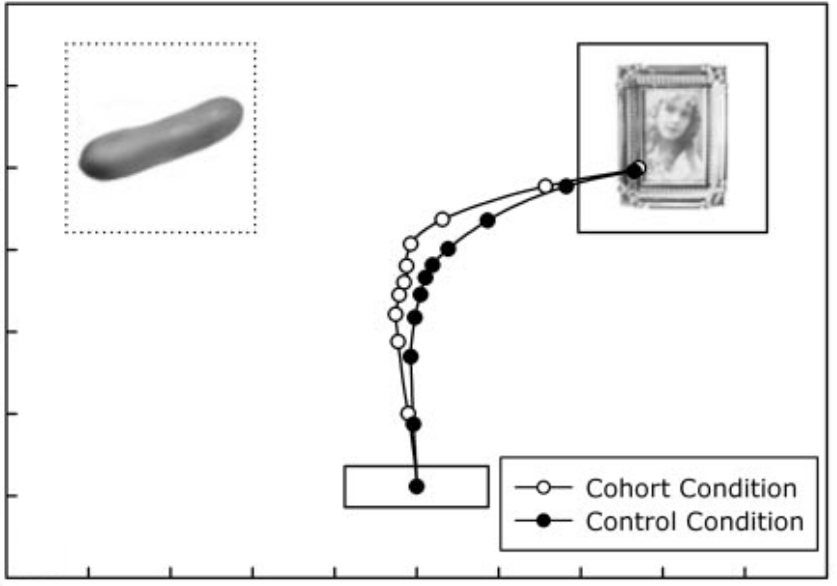
\includegraphics[width=.7\textwidth]{../1.Conflict/imgs/spivey.png}
  \caption[\citegap{Spivey2005}{'s} mouse tracking paradigm.]{
    \citegap{Spivey2005}{'s} mouse tracking paradigm.
    Participants were told aurally to click on the ``picture''.
    Their mouse cursor trajectories showed a greater, graded attraction
    towards the alternative icon in the cohort (conflict) condition,
    where it showed a phonological competitor (a pickle), than in the control condition,
    where it did not.
    \label{fig:chapter2-spivey}
  }
\end{figure}

In the years since its introduction,
this paradigm has been adapted for a range of problems.
Unsurprisingly, there has been considerable diversity in these subsequent mouse tracking studies,
in terms of specific details of the experiment itself,
the processing and analysis of dependent variables,
and the nature of the results obtained.
In the next section, I review previous mouse tracking work along these lines,
and outline the procedure as used in the later experimental chapters of this thesis.
By covering this material here, we are saved from repeating
many of the technical details for each experiment.

% Other mouse tracking
As discussed in Chapter 1,
this is not the only mouse tracking paradigm used in behavioural research.
However, in this review, I will focus on the two-option forced choice
mouse tracking design introduced  by \citet{Spivey2005}.


\subsection{Procedure}\label{sec:chapter2-mousetracking-procedure}

The canonical mouse tracking procedure differs little
from that used by \citet{Spivey2005}.
Two response options are located in the top corners of the screen,
and participants click on a start button 
located in the bottom of the screen to begin a trial.
After this, and usually following a fixation cross,
stimuli are presented, either visually or aurally,
and participants move the mouse cursor from its starting point
to click on one or other response option.

% Specifics of our version
Naturally, for mouse tracking to be useful,
participants must begin moving the cursor
before they have fully made up their minds on each trial.
Following \citet{Freeman2009}, it is common practice
on trials where the mouse cursor isn't moved within a given time from
stimulus onset \citep[400 msec in][]{Freeman2009}
to show participants a message asking them to
start moving earlier, even if they weren't fully certain of their response.
The length of this window obviously varies between tasks,
as participants may simply refuse to move too early 
for more difficult decisions.
In the experiments reported here, the maximum initiation window
for each experiment was decided based on pilot testing.
\citet{Scherbaum2010} offer a different solution to this problem
by programming their experiment to only reveal the stimuli
once participants began their mouse movement.
However, this technique does not appear
suitable for the more complex experiments reported in this thesis.

In designing the experiments here,
I have developed a technique which may prove useful 
for readers interested in adopting these methods,
of encouraging mouse movements during the decision process.
Through pilot testing,
it is possible to estimate a reasonable amount of time
for participants to be able to 
initiate their response movements for a given experiment.
Having identified a desired initiation time (for instance, 500 msec),
the duration of the fixation cross is set to three times this,
that is, a blank screen for 500 msec,
a cross for 500 msec,
and a blank screen for 500 msec,
followed by onset of the stimuli.
This creates a ready-set-go effect,
and encourages participants to attempt to synchronise
the onset of their own movement to this interval.

Another variable is the maximum amount of time allowed to respond.
For many simple experiments, such a limit is unnecessary,
as participants respond within 2 to 3 seconds without extra prompting.
For more complex experiments, and certainly for reasoning, however,
self-paced participants would be likely 
to take considerably longer than this to respond,
and so their decisions would not be captured in their mouse movements.
In addition, to require early movement initiation,
without speeded responses,
would incentivise participants to move the cursor around the screen
as they made their decisions an in undesirable fashion.
Therefore, most of the experiments reported here 
required participants to respond within a certain time window,
the length of which was again decided upon after pilot testing.


% Feedback?

% Resetting Mouse cursor

A fine detail in these experiments is 
the location of the cursor on stimulus onset.
In the majority of experiments, this is controlled by the software:
after clicking on the start button,
a fixation cross is typically displayed before stimulus onset,
and the cursor position is reset to the bottom centre of the screen
if it has moved during the fixation period.
In the experiments reported herein,
two different sets of software are used for different experiments,
one written in python, and one run in the web browser (see below).
At present, it is not possible to manipulate 
the position of a mouse cursor in the browser,
and so in the experiments which used this software
it was not possible to reset the cursor position.
This issue was circumvented in these particular experiments
by using very short fixations, or no fixation at all.

% Stimuli presentation

In mouse tracking experiments, attention must also be given to
the way in which information is presented to participants
during a trial.
Most experiments use simple stimuli,
such as images or text, which can be presented to participants simultaneously.
In reasoning experiments, however, it is often necessary
to present participants with much more information.
My initial attempts to present entire reasoning problems at once
revealed that participants would first processes all of the stimuli,
over several seconds, and only after making their decision
move the mouse cursor.
Therefore, great care was taken 
to present participants with stimuli on each trial
in such a way that they had sufficient time 
to process all of the contextualising information.
Trials were structured so that it was not possible
to begin making a decision until the onset of the final stimuli, 
so that the movement of the mouse cursor could capture this process.
For instance, in Experiment 3,
an inductive reasoning task,
participants were presented with a property,
told that it can be found in one of two species,
and shown each of the candidate responses 
in their locations in the top corners of the screen, one at a time.
Only after this information was presented could participants
click on the start button, which caused the base species,
which was known to have the property in question,
to be shown in the centre of the screen.
At this point, participants used this new information
to decide which of the candidate species
was more likely to possess the property.


\subsection{Stimuli}\label{sec:mousetracking-stimuli}

Typically, mouse tracking experiments use one of two manipulations.
One option is to manipulate, between conditions, the probe to which participants respond.
In \citet{Freeman2008}, participants were shown
computer-generated male and female faces which were either gender typical or typical,
while the response icons remained constant: MALE, and FEMALE.
The alternative is to manipulate the possible responses.
For instance, \citet{Spivey2005} presented the probe word ``pickle'' twice:
once when the foil response was a phonological competitor (a PICTURE)
and once when it was not (a CANDY).

This distinction may be important, as in the former case
the experimental manipulation changes the relationship between
the probe and the chosen response,
and so it is difficult to disentangle an effect driven by conflict,
and an effect driven by reduced confidence in the response.
In the latter case, the link between the probe and the response remain the same,
and so any changes in motor output
must be a result of an attraction towards the distractor response.
\citet{Dale2007} demonstrate the value of combining these approaches.
In their first experiment, they showed that
as participants categorised animals into their super-ordinate categories (i.e. WHALES as MAMMALS),
they showed greater mouse curvature for atypical category members (WHALES)
than typical ones (COWS).
However, this effect could be simply due to
reduced confidence in the chosen response, rather than conflict per se.
To show that this was a conflict effect,
they ran  a follow-up experiment showing that the effect was diminished
when the distractor was not associated with the probe item
(i.e. BIRDS, instead of FISH, for WHALES).
Another possible implication of this distinction,
which is yet to be fully investigated,
is that when the distractor response is the independent variable
participants could plausibly be faster to execute some aspects of their responses under conflict.
Although their reasons for choosing the dominant response remain the same,
the conflict condition in such experiments provides
an additional reason to initiate a response,
and so movement initiation may paradoxically be faster under conflict.
In this thesis, I use both kinds of manipulation.


\subsection{Software}\label{sec:mousetracking-software}

A number of tools are available for running mouse tracking experiments,
and processing the resulting data.
MouseTracker 
\citep[\href{http://www.mousetracker.org/}{www.MouseTracker.org};][]{Freeman2010a},
the most popular option,
provides a graphical experiment builder,
and a point-and-click interface for 
calculating relevant summaries of trajectories (discussed below)
and exporting them for analysis.
While MouseTracker was initially used in this research,
and should be recommended for researchers interested in exploring mouse tracking,
it sacrifices a certain amount of flexibility for ease of use,
and so proved to be inadequate for the complex reasoning paradigms
used in this thesis.

I developed two tools to solve this problem.
First, I implemented the paradigm
as a script in the python programming language,
and ran it using the open source OpenSesame experiment builder \citep{Mathot2011a}.
This implementation, along with detailed instructions,
are available online at
% \href{https://github.com/EoinTravers/QuickstartMousetracking}{
%   github.com/EoinTravers/QuickstartMousetracking}.
\hspace*{4pt}\url{https://github.com/EoinTravers/QuickstartMousetracking}.
I also created a second implementation of the paradigm as part of
PsychScript
(\url{https://github.com/EoinTravers/PsychScript}),
a set of tools I have written in HTML, JavaScript, and PHP
for running behavioural experiments online in the web browser.
Both implementations of the mouse tracking paradigm were extremely similar,
and differed principally in that 
it was not possible to manipulate 
the position of the mouse cursor using PsychScript, 
and so its location was not reset on experiments implemented using this platform
(see above).
Although it was possible to run experiments
programmed using PsychScript outside the laboratory (that is, online),
this capability was only used for pilot testing
due to concerns about the quality of data collected in this way.
Instead, this implementation was primarily used
to collect data in undergraduate computer laboratory classrooms,
as it made it possible to recruit large numbers of participants at once
without the necessity of installing OpenSesame on each computer.

MouseTracker automatically calculates a number of statistics
for describing mouse cursor trajectories
to be used in later analyses (see below).
Using my own implementations of the paradigm,
it was also necessary to write code to calculate these same measures.
This was done in the python programming language,
and released as the python package Squeak
(\url{https://github.com/EoinTravers/Squeak}).
A guide to using Squeak can be found alongside
my python implementation of the mouse tracking procedure,
at \url{https://github.com/EoinTravers/QuickstartMousetracking}.




\section{Analysing Mouse Data}\label{sec:mousetracking-analysing}

Even for simple experiments, mouse tracking creates a voluminous amount of data.
As a result, there are many ways in which data from these experiments can be analysed.
In general, however, two strategies are popular:
each trials' trajectory can be reduced to a single summary measure,
or the actual time course of trajectories across conditions can be analysed.
While space precludes a review of all measures used in this kind of research,
in this next section I will outline the measures used in the present studies,
and the motivation behind their choice.

% Summary statistics
The simplest summary measure, of course, is response latency, or response time (RT),
which works the same way for mouse tracking
as it does in other paradigms:
the time between stimulus onset and a response.
This can be accompanied by a measure of movement initiation time (IT),
reflecting the time from stimulus onset
to the cursor beginning to move.
In the current studies, IT was defined as the time taken
for the cursor to move 1\% of its total distance travelled vertically.

\begin{figure}[ht]
  \centering
  \includegraphics[width=\figurewidth]{imgs/cursor_measures.pdf}
  \caption[Summary measures for cursor trajectories.]{
    \label{fig:cursor_measures}
    For analysis, mouse cursor trajectories are remapped to a standard co-ordinate space,
    beginning at $[0,0]$ and ending at $[1,1.5]$.
    Area Under the Curve reflects the size of the region bounded by this trajectory
    and an ideal straight line from start to finish,
    in the dimensions of the standard co-ordinate space.
    Maximum Deviation is the greatest perpendicular distance
    between the ideal straight line
    and the actual trajectory.
  }
\end{figure}


More interesting, however, are measures derived from
the shape of the trajectory followed by the cursor.
For these, as in all subsequent analyses of cursor movements,
each trajectory is mapped on to a common co-ordinate system,
such that they begin at point $[0,0]$ (the bottom centre),
and end at point $[1,1.5]$ (the top right corner;
see Figure~\ref{fig:cursor_measures}).
Trajectories which finished in the top left corner
are usually reflected on the y axis 
so that all trials end at the same point,
although in analyses including both correct and incorrect responses
the original endpoint of $[1,-1.5]$ may be used as 
the location of the incorrect response option.
\citet{Spivey2005} quantified the curvature of their cursor trajectories
using a measure of Area Under the Curve (AUC),
corresponding to the area bounded between the actual trajectory
and a straight line between its start and end points
(again, see Figure~\ref{fig:cursor_measures}).
Complications arise, however,
when we attempt to calculate AUC for trajectories which contain loops,
or those which pass on the other side of the idealised straight line
(closer to the edge of the screen),
as the treatment of such cases varies depending on the algorithm used,
and no standard has been established among mouse tracking researchers.
While such trajectories were apparently rare
in studies of simple perceptual judgements
and could be excluded from analyses,
they have proven more common in my work on reasoning,
and so I do not make use of AUC in this thesis.

A commonly used alternative to AUC is
the Maximum Deviation (MD) of a trajectory,
the greatest distance achieved between the trajectory
and the idealised straight line (again, see Figure~\ref{fig:cursor_measures}).
In conversation with other researchers interested in mouse tracking,
it has also become apparent that 
there is more than one way to calculate this.
For clarity, MD is calculated in this thesis
by rotating a trajectory by $\tan^{-1}( \frac{1.5}{1} )$
(approximately $56^{\circ}$) clockwise 
so that its ideal straight line follows the x axis.
MD is then simply the greatest height of 
the rotated trajectory on the y axis.
MD can be negative:
trajectories which stray further from the straight line to the right
(towards the edge of the screen)
than to the left (towards the alternative response)
will have MDs of less than 0.
Some variations have been proposed on this measure,
including Maximum Absolute Deviation,
in which these negative values are treated as positive,
and Average Absolute Deviation,
which takes the mean of the absolute deviation
across the time course of trial \citep{Koop2013}.
However, I have opted for MD as my preferred measure,
largely because it is the most commonly used measure of deviation.


Other measures reflect the complexity of cursor movements,
indicating either conflict, or at very least uncertainty
\citep{Wojnowicz2009, Dale2011}.
X-flips (changes of direction on the x axis)
over the course of a trajectory, provide one such measure,
although it is not always clear what this statistic reflects,
as zig-zags across the entire screen
and wobbles over a few pixels
both constitute changes of direction.
Alternatively, it is possible to calculate the number of
acceleration components -- 
changes from acceleration to deceleration, and vice versa --
during a trial as a measure of movement complexity
\citep{Dale2011}.
An interesting alternative measure of complexity 
is sample entropy, \citep{Richman2000, Dale2007}
which reflects the amount of extra information
imparted at every time point in a trajectory.
However, I do not make use of these measures in this thesis.


\subsection{Continuous and Discrete Effects} \label{sec:mousetracking-continuous}

Unlike eye movements, which are ballistic in nature,
and so (almost) always move in a straight line from their starting point to their destination,
hand movements can follow any number of trajectories.
Thus, the mouse tracking paradigm can also reveal
something of the qualitative nature of conflict as it unfolds.
In Chapter 1, I discussed two ways conflict has been seen in mouse tracking.
Most studies have found continuous attraction effects,
where participants are initially drawn towards both response options,
but gradually home in one or other of them,
following a graded curve of the type seen in Figure~\ref{fig:cursor_measures}.
Some studies, however, have found discrete effects,
where participants sometimes move directly to their response,
but other times initially move in one direction,
but change their mind, and change direction, mid-trial.
In Appendix~\ref{appendix:mouse-studies},
I list studies in which each kind of effect has been found.

To tease these possibilities apart,
it is necessary analyse the distribution of trajectories in an experiment
\citep{Spivey2005,Freeman2012}.
While these points also apply to the trajectories themselves,
for practical purposes these analyses usually focus on
summary measures, such as AUC or MD.
In cases of continuous attraction, according to this logic,
we should find that most trajectories are slightly curved,
and that the average curvature is greater for conflict trials.
Statistically, this equates to data where MD is normally distributed within each condition,
and the mean of this distribution is higher for conflict trials.
In cases of discrete attraction, however,
there are some trajectories which go straight to an option, with very little curvature,
and some which initially go one way, and then change direction, with high curvature.
Statistically, this leads to MD being bimodally distributed,
with the direct trajectories forming a sub-population with MD close to $0$,
and the reversals, or changes of mind, forming a sub-population with a much higher mean MD
(Figure~\ref{fig:exp2-reversals-in-chap}).

To test for bimodality in their data,
\citet{Spivey2005} calculated the Bimodality Coefficient \citep[BC;][]{SASInstitute1990}:

\begin{equation}
  BC = \frac
  {m_3^2 + 1}
  {m_4 + 3 \times \frac{(n-1)^2}{(n-2)(n-3)}}
\end{equation}
where $n$ is the sample size, $m_3$ the skewness, and $m_4$ the excess kurtosis
\citep[see][]{Pfister2013,Freeman2012}.
A uniform distribution has BC of .555,
and so values higher than this constitute evidence of bimodality.
\citet{Spivey2005} also supported their interpretation,
although this method has not been widely adopted,
by comparing the distributions of the conflict and control conditions
using the Kolmogorov–Smirnov test.
Finding that there was no significant difference in
the shape of the distributions between conditions,
they concluded that the greater AUC under conflict
was not the result of a subset of high AUC trials.
\citet{Freeman2012} provided a more in-depth analysis of tools
for distinguishing between unimodal and bimodal distributions,
and recommend, based on simulation results, the use of
Hartigan's Dip Statistic \citep{Hartigan1985}.
This measure tests the null hypothesis that
the data is unimodally distributed,
and so $p < .05$ indicates that the data is significantly bimodal.
In this thesis, I make use of both BC
and Hartigan's Dip Statistic when analysing distributions.

In all of the experiments reported in Chapters 3, 4, and 5,
I find evidence of discrete attraction:
some trials move directly towards the correct response option,
some initial move towards the wrong option before redirecting,
while some give the wrong response (see Appendix~\ref{appendix:reversals}).
It is difficult, from a statistical perspective, to analyse such data,
as most analyses require normally distributed residuals,
and unlike in the case of skewed data such as response latencies,
there is no transformation to map bimodal data
onto a normal distribution.
Therefore, I instead class each trajectory
as being either direct (from the low-MD sub-population)
or a reversal (from the high-MD sub-population),
and use the proportion of reversals in each condition
as my dependent variable.

To classify trajectories in this way,
I use two-sample finite mixture models,
modelling the MD distribution as two normally distributed sub-populations,
and derive from this a cut-off value.
MDs below this value are classed as direct movements,
and those above it as reversals.
I have chosen this approach, rather than others such as the k-means algorithm,
as unlike k-means, finite mixture models allow for differences in variability
between the two sub-populations:
we would expect less variability in direct movements to the response
than in reversals, and this is confirmed in the data.
Figure~\ref{fig:exp2-reversals-in-chap} shows this procedure
as conducted for Experiment 2.
Appendix~\ref{appendix:reversals} shows details of this procedure
for each of Experiments 1 to 5.

\begin{figure}[ht]
  \centering
  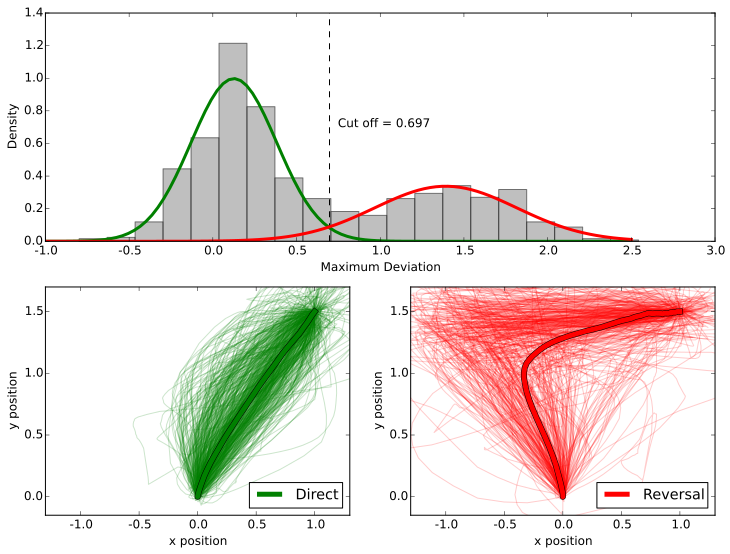
\includegraphics[width=.8\textwidth]{../Appendices/imgs/reversals/exp2-reversals}
  \caption{
    \label{fig:exp2-reversals-in-chap}
    Trajectories classed as direct and reversals in Experiment 2.
  }
\end{figure}


\subsection{Types of Trajectory}

In these mouse tracking experiments, 
participants chose either the correct option or the foil,
and either traced a direct path, or changed direction while doing so.
In this sense, setting aside questions of \emph{when} each movement occurs,
there are four kinds of responses, or trajectories,
possible in such experiments:
direct movements to the correct response,
reversals ending with the correct response,
direct movements to the foil,
and reversals ending with the foil (see Figure~\ref{fig:trajectory-types}).
It is illustrative to analyse how the proportion of each trajectory
changes between conditions in an experiment,
and I do so for Experiments 1 to 5.

Perhaps a more interesting analysis, however,
is to look to the decisions participants could make
over the course of a single trial.
I assume that participants make two decisions on each trial.
First, at the onset, they must decide to move
either towards the correct option,
the probability of which I will denote as $\alpha$,
or to move towards the foil, with probability $1 - \alpha$.
If they do initially move towards the correct option,
they may subsequently select this option,
with probability $\beta$,
or change direction and select the foil option instead,
with probability $1 - \beta$.
Finally, if they initially move towards the foil,
they may still change direction and chose the correct option,
with probability $\gamma$,
or otherwise persevere to the foil option,
with probability $1 - \gamma$.
These probabilities are illustrated in Figure~\ref{fig:trajectory-types}.
Note that for each decision,
the labelled probabilities ($\alpha$, $\beta$, and $\gamma$)
denote the probability of moving towards or selecting the correct option,
while their compliments  ($1 - \alpha$, $1 - \beta$, and $1 - \gamma$)
denote the probability of moving towards or selecting the foil.
Equation~\ref{eq:transitions} summarises
the definitions of each of these probabilities.

\begin{equation}
  \label{eq:transitions}
  %% You don't caption equations!
  %% \caption{
  %%   Transition probabilities $\alpha$, $\beta$, and $\gamma$
  %%   for describing cursor trajectories.
  %%   $\alpha$ is the probability of initially moving towards the correct option,
  %%   $\beta$ of selecting the correct option after initially moving towards it,
  %%   and $\gamma$ the probability of selecting the correct option
  %%   after initially moving towards the incorrect foil option.
  %% }
  \begin{split}
    \alpha &= P(Initially\ correct)\\
    \beta  &= P(Correct\ response | Initially\ correct)\\
    \gamma &= P(Correct\ response | Initially\ incorrect)
  \end{split}
\end{equation}


\begin{figure}[ht]
  \centering
  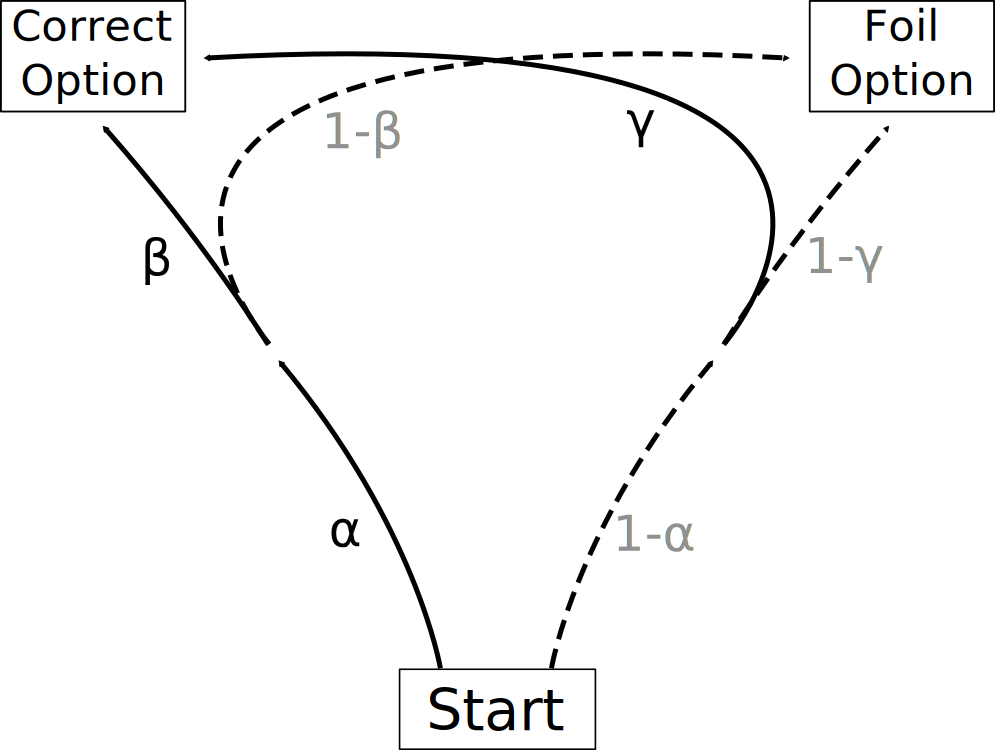
\includegraphics[width=.6\textwidth]{imgs/transitions.pdf}
  \caption[Parameters for descriptions cursor transitions.]{
    \label{fig:trajectory-types}
    Mouse trajectories in a given condition can be described in terms of
    the probability of initially moving toward the correct option ($\alpha$),
    the probability of choosing the correct option
    after initially moving towards it ($\beta$),
    and the probability of choosing the correct option
    despite initially moving towards the foil ($\gamma$).
  }
\end{figure}








\subsection{Time course}

Beyond the shape of cursor trajectories,
we can analyse their time course.
Unsurprisingly, there has also been considerable variation
in how these time series data are used in the literature.
% Normalised or Raw time
\citet{Spivey2005} introduced the convention, 
still used in most studies,
of standardising the time course of trajectories of different durations
by interpolating them to 101 discrete time points,
corresponding to the location of the cursor 
from 0\% to 100\% of the way through the trial.
While this approach somewhat simplifies further analyses,
it is problematic in the current research;
when there is considerable variation in response latencies,
the 50\% point may be significantly later in one condition than another,
and so it would be misleading to compare
the location of the cursor at this point between conditions.
An alternative approach, which I use instead,
is to use the real time information,
specifically the location of the cursor every 20 msec through the trial.
As standard computer mice typically update their position
every 10-15 msec, this frequency strikes a balance between
temporal precision and oversampling of the data.

% Plotting
Most mouse tracking studies include some form of plot
showing the average cursor trajectories in each condition.
However, for the experiments reported here
--- every one of which revealed discrete attraction effects ---
to do so would be misleading.
As noted by \citet{Spivey2005}, if we average
trajectories from conditions where
some trials initially go towards the alternative option
and other go straight to the correct one,
or if we average trajectories from conditions where
all trials were moderately curved,
in both cases we end up with a mean trajectory that follows a smooth curve,
like those shown in Figures~\ref{fig:chapter2-spivey} and \ref{fig:cursor_measures}.
However, such an average trajectory would be a misleading description
of the kind of data I find in this thesis,
as few trials actually follow such a gently curving trajectory
(see Figure~\ref{fig:average-cursor}).

Instead, I opted to match these discrete attraction effects
with a discrete analysis.
For every 20 msec window, from every trial,
I classed the cursor as being either
in its starting position,
on the side of the screen containing the correct option,
or on the side containing the foil.
I then investigated the proportion of trials
on each side of the screen, over time.

Beyond visualisation, researchers usually wish to
perform some kind of inference with these data.
A crude, but simple method of assessing when conflict occurs,
again introduced by \citet{Spivey2005},
is to conduct a series of t tests, 
usually on the 101 normalised time steps,
but also possibly on the real-time data,
comparing the x axis position between conditions at each time step,
and noting the window for which the difference is significant.
Although this approach does not provide
a valid significance test for comparing conditions in general,
it does provide an easily interpretable indication of
\emph{when} participants are drawn towards a competing response.
It is possible, but rarely done in practice,
to derive by means of simulations
the likelihood of achieving a run of significant differences 
of length $n$ under the null hypothesis \citep{Dale2007},
and thus calculate a valid p value for the difference between conditions overall.
A similar analysis has also been reported 
calculating at each time step
the distance between the cursor and the non-chosen response,
and comparing this between conditions \citep{Falke2013}.

\begin{figure}[ht]
  \centering
  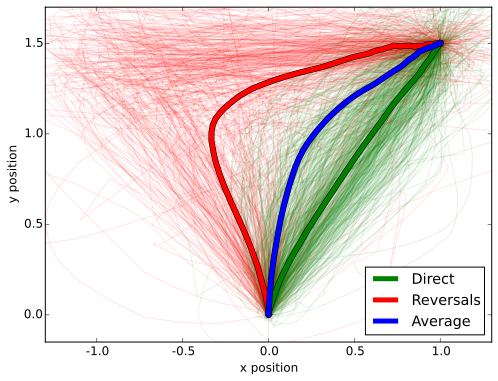
\includegraphics[width=\figurewidth]{imgs/exp2-average-cursor}
  \caption[The pitfalls of averaging cursor trajectories.]{
    \label{fig:average-cursor}
    Averaging direct trajectories (green) and reversals (red)
    produces an aggregate trajectory that appears to curve gently.
    However, few of the actual trajectories curve in this way.
    These data come from Experiment 2 (Chapter 3).
  }
\end{figure}


Again, though, the experiments reported here
reveal discrete movements towards one or other response option,
with reversals on some trials,
rather than the graded, curved trajectories seen in much previous work.
Therefore, an averaged trajectory is an inappropriate measure,
as it falls somewhere between the direct trajectories and the reversals
(see Figure~\ref{fig:average-cursor}).
For this reason, in Experiments 1 to 5
I instead code the location of the cursor over time on each trial
as being either on
the side of the screen corresponding to the correct option,
or the side corresponding to the foil
(excluding cases where the cursor is yet to be moved).
I then compared, in every 20 msec window,
the probability of being on either side of the screen to chance,
or the probability of being on one or other side between conditions,
using logistic mixed effects models (see below).
Attraction towards the foil option is therefore revealed by
an increase in the proportion of trials
where the cursor is on that side of the screen.

In line with previous mouse tracking studies,
for each time course analysis I run a series of comparisons,
one on each 20 msec time slice,
and report the times from which significant effects emerge and disappear.
Instead of t tests, however, I use logistic mixed models,
for reasons outlined below.

Finally, an alternative to running a series of comparisons
is to fit polynomial regression models, or \emph{growth curves},
to the time course data
(\citealp{Falke2013};
 \citealp[see][for an introduction to this method in eye tracking research]{Mirman2014}).
These are regression models in which time,
and often polynomial terms such as time$^2$ and time$^3$,
are included as predictors.
Such models are often used to model changes in subjects over time,
such as the change in height of a child over a number of months, hence their name.
Growth curves are discussed in detail in Chapter 6.


